\documentclass[a4paper,norsk]{article}
\usepackage{preamble}
\usepackage{tabu}
\usepackage{color, colortbl}
\definecolor{LightCyan}{rgb}{0.88,1,1}

\begin{document}
\maketitle
We let $((x_k, y_k, z_k))_{k=1}^m$ be some avaulable data points in $\mathbb{R}^3$, and we want to define a model based on a smaller set of 
coordinates ${(u_j, v_j)}_{j=1}^n$ in $\mathbb{R}^2$. As mentioned in the introduction $(u_j, v_j)$ will be the vertices of the triangles moddeling the the set of
data points. Further we define piecewise linear functions ${N_j(x, y)}_{j=1}^n$ such that $N_j(u_j, v_j) = 1$, $N_j(u_i, v_i) = 0$ if i $\neq$ j. These functions are mutch alike the "hat functions" found in the Finite Element method. Our goal will be to find a least squares fit to approximate the given dataset with these functions.

\section*{Exercise 1}
\begin{figure}[h!]
	\centering
	\caption*{\textbf{Visualization of a piecewise linear function $N_j$ \newline (Figure from MEK4250 course book)}}
	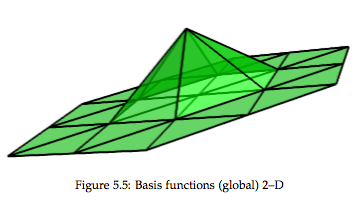
\includegraphics[scale=0.36]{element.png}
\end{figure}

Deriving the matrix spanning the functions $N_j$ defined as B in the mandatory exercise we see that 
\begin{align}
\text{\textbf{B}} = 
\begin{pmatrix}
 N_1(x_1,y_1) & N_2(x_1,y_1) & \cdots & N_n(x_1,y_1) \\
 N_1(x_2,y_2) & N_2(x_2,y_2) & \cdots & N_n(x_2,y_2) \\
 \vdots  & \vdots  & \ddots & \vdots  \\
 N_1(x_m,y_m) & N_2(x_m,y_m) & \cdots & N_n(x_m,y_m)
 \end{pmatrix}
\end{align}

Now let us assume that at least two ${u_j, v_j}$ are located at the same point, say $j = 1,2$. Then by definition $N_1(u_1, v_1)$ and $N_2(u_2, v_2)$ will be defined over same area with the same properties as introduced. Hence we end up with two equal columns in the \textbf{B} matrix, and we ha a linear dependent system. Therefore we can assure that the functions ${N_j(x, y)}_{j=1}^n$ are linearly independent as long as ${u_j, v_j}_{j=1}^n$ are located at different points.

\newpage
\section*{Exercise 2}
Moving on, we want to show that if we choose our $(u_j, v_j)$ among our data points $(x_j, y_j)$, then the columns of \textbf{B} are linear independent. This 
\textbf{B} matrix is defined from the least squares system trying to fit our datapoints $((x_k, y_k, z_k))_{k=1}^m$ using the defined functions $N_j$. The squared
error is defined as 

\begin{align*}
\sum_{k=1}^m \Big(\sum_{j=1}^n c_j N_j(x_k, y_k) - z_k  \Big)^2 = {||\textbf{Bc} - \textbf{z} ||_2^2}
\end{align*}
Where \textbf{B} is our coefficient matrix as defined in task 1. \\
I don't know if I have misunderstood something critical in the argument, but from my point of view it seems that the answer follows directly from our result in task 1. It is reasonable to assume that the data points $(x_j, y_j)$ don't have any equal points. By this assumption we can always choose some $(u_j, v_j)$ 
from $(x_j, y_j)$ such that none of these are located at the same point. Then from task 1, we can argue that the matrix \textbf{B} is linear independent, which follows that there exists a unique least squares solution.

\section*{Exercise 3}
Now let's say that for some j, the triangles sharing $(u_j, v_j)$ as a vertex doesn't contaion any datapoints. In other words for this j our our data points are only located where this $N_j = 0$. Think of it as from our figure in task 1, the points are located "outside" where this function $N_j$ has its linear properties.
By this observation the function $N_j$ will only give 0 contributions to its column in the \textbf{B} matrix, yeilding and linearly dependent system.  

\newpage
\section*{Exercise 4}
This simple program writes out the barycentric coordinates of \textbf{p}, relative to the trangle spanned by $\textbf{p}_1$, $\textbf{p}_2$ and $\textbf{p}_3$. 
A simple run set by the coordinates $\textbf{p}_1 = (0, 0)$, $\textbf{p}_2 = (1, 1)$, $\textbf{p}_3 = (-1, 1)$ for $\textbf{p} = (0.5, 0)$ yeilds

\begin{lstlisting}[style=terminal]
Find the barycentric coordinates of (0, 0.5) 
In the triangle spanned by 

p1 = [0, 0]
p2 = [1, 1]
p3 = [-1, 1]

The barycentric coordinates of p relative to the spanned triangle:
b1 = 0.5,  b2 = 0.25,   b3 = 0.25
\end{lstlisting}

\begin{lstlisting}[style=python]
import numpy as np

def barycentric(p1, p2, p3, p):
    #barycentric takes 4 arguments.
    #p1, p2, p3 are the points spanning the triangle, 
    #hence these must not lie on a line
    #p is the point within the triangle

    print "Find the barycentric coordinates of (%g, %g) \n" \
    "In the triangle spanned by \n" % (p[0], p[1])
    count = 1
    for i in [p1, p2, p3]:
        print "p%d = [%g, %g]" % (count, i[0], i[1])
        count += 1

    cond = [1 for i in range(3)]

    #Assemble the left hand side of the system
    A =  np.vstack([p1, p2, p3])
    A = np.append(np.transpose(A), [cond], axis=0)

    #Assemble the right hand side of the system
    L = np.insert(np.array(p), len(p), 1)

    #solve system
    b = np.linalg.solve(A, L)

    #Print result
    print "\nThe barycentric coordinates of p relative to the spanned triangle:"
    print "b1 = %g,  b2 = %g,   b3 = %g" % (b[0], b[1], b[2])

p1 = [0, 0]
p2 = [1, 1]
p3 = [-1, 1]

p = [0, 0.5]

barycentric(p1, p2, p3, p)
\end{lstlisting}

\newpage
\section{Exercise 5}




\end{document}
